\section{Materialers beteende}

\paragraph{Idealplastisk deformation}
De flesta material beter sig så att när de deformeras förbi en viss punkt, deformeras de plastiskt i stället för elastiskt. En approximation för att beskriva detta beteendet är att låta deformationen vara elastisk upp till en töjningsgräns $\varepsilon_{\text{s}}$, och låta $\sigma$ vara konstant lika med en sträckgräns $\sigma_{\text{s}}$ för större töjningar.

När lasten sedan tas bort, kommer stången förkortas igen tills lasten blir lika med noll. Denna kontraktionen är parallell med det elastiska regimet, och konsekvensen är att man får en permanent deformation.

\paragraph{Enkelriktad fiberkomposit}
En enkelriktad fiberkomposit är ett material som består av fibrar som alla är parallella och ett omkransande material som kallas en matris. Matrisen och fibern finns i volymfraktioner $v_{\text{m}}$ respektiva $v_{\text{f}}$, och de har elasticitetsmoduler $E_{\text{m}}$ respektiva $E_{\text{f}}$.

Som en modell för belastning längsmed fibrernas riktning betraktar vi uppställningen som ges i figur \ref{fig:fiber_composite_parallel}.
\begin{figure}[!ht]
	\centering
	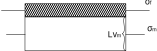
\includegraphics[width = 0.5\textwidth]{./Images/fiber_composite_parallel.eps}
	\caption{Illustration av en del av en enkelriktad fiberkomposit som belastas längsmed fiberns riktning.}
	\label{fig:fiber_composite_parallel}
\end{figure}

Kraftjämvikten ger $F = \sigma A$. Vi antar att den utskurna biten är ett rätblock, så de två delarna har tvärsnittsareor som ges av totala tvärsnittsarean och volymfraktionerna. Detta ger
\begin{align*}
	F = \sigma A = (\sigma_{\text{f}}v_{\text{f}} + \sigma_{\text{m}}v_{\text{m}})A.
\end{align*}
Därmed ges spänningen av
\begin{align*}
	\sigma = \sigma_{\text{f}}v_{\text{f}} + \sigma_{\text{m}}v_{\text{m}}.
\end{align*}
Vi antar att fibern och matrisen inte glider relativt varandra, och därmed har de samma deformation och töjning. Hookes lag ger
\begin{align*}
	\sigma_{\text{f}} = E_{\text{f}}\varepsilon, \sigma_{\text{m}} = E_{\text{m}}\varepsilon,
\end{align*}
vilket insatt i uttrycket ovan ger
\begin{align*}
	\sigma &= v_{\text{f}}E_{\text{f}}\varepsilon + v_{\text{m}}E_{\text{m}}\varepsilon \\
	       &= (v_{\text{f}}E_{\text{f}} + v_{\text{m}}E_{\text{m}})\varepsilon.
\end{align*}
För hela biten med fiberkomposit ger Hookes lag då
\begin{align*}
	E_{\text{L}} = v_{\text{f}}E_{\text{f}} + v_{\text{m}}E_{\text{m}}
\end{align*}
som elasticitetsmodulen vid längsgående spänning. Vi får även
\begin{align*}
	\sigma_{\text{f}} &= E_{\text{f}}\varepsilon \\
	                  &= \frac{E_{\text{f}}}{E_{\text{L}}}\sigma
\end{align*}
som spänning i fibrerna, och motsvarande för matrisen.

På samma sättet beskriver vi även fallet när spänningen går på tvärs av fibrernas riktning, som illustrerad i figur \ref{fig:fiber_composite_normal}.
\begin{figure}[!ht]
	\centering
	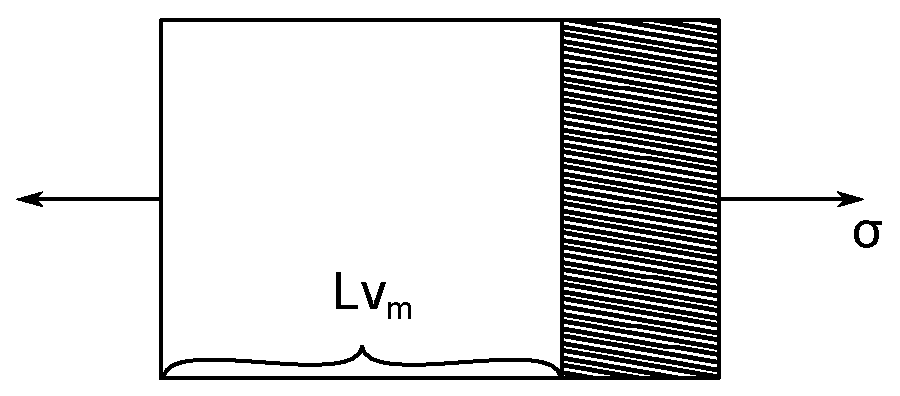
\includegraphics[width = 0.5\textwidth]{./Images/fiber_composite_normal.eps}
	\caption{Illustration av en del av en enkelriktad fiberkomposit som belastas normalt på fiberns riktning.}
	\label{fig:fiber_composite_normal}
\end{figure}

Här kan vi snitta och se att $\sigma_{\text{f}} = \sigma_{\text{m}}$. Den totala förlängningen i denna biten ges av
\begin{align*}
	\delta = \delta_{\text{f}} + \delta_{\text{m}} = L_{\text{f}}\varepsilon_{\text{f}} + L_{\text{m}}\varepsilon_{\text{m}}.
\end{align*}
Töjningen ges då av
\begin{align*}
	\varepsilon &= \frac{\delta}{L_{\text{f}} + L_{\text{m}}} \\
	            &= \varepsilon_{\text{f}}\frac{L_{\text{f}}}{L_{\text{f}} + L_{\text{m}}} + \varepsilon_{\text{m}}\frac{L_{\text{m}}}{L_{\text{f}} + L_{\text{m}}} \\
	            &= v_{\text{f}}\varepsilon_{\text{f}} + v_{\text{m}}\varepsilon_{\text{m}}.
\end{align*}
Hookes lag ger
\begin{align*}
	\varepsilon &= v_{\text{f}}\frac{\sigma}{E_{\text{f}}} + v_{\text{m}}\frac{\sigma}{E_{\text{m}}},
\end{align*}
och vi ser att
\begin{align*}
	\frac{1}{E_{T}} = \frac{v_{\text{f}}}{E_{\text{f}}} + \frac{v_{\text{m}}}{E_{\text{m}}}.
\end{align*}

\paragraph{Ideallastisk vridning}
Vi inför idealplastiska material även i vridningssammanhang. Dessa beter sig analogt till idealplastiska material under dragning, där vi ersätter töjningen med skjuvvinkeln $\gamma$, spänningen med skjuvspänningen $\tau$, töjningsgränsen med en vinkelgräns $\gamma_{\text{s}}$ och sträckgränsen med en skjuvgräns $\tau_{\text{s}}$.